\section{Model Learning \& Optimization}

\begin{frame}
\frametitle{Mobile Robot Navigation}
\textcolor{tudblue}{\textbf{Goal:}} Move robot to area while minimizing traveled distance
\vfill

\begin{columns}[T]
\begin{column}{0.5\textwidth}
\onslide<2->{
MDP Model $\mathcal{M}$ should define:
\begin{itemize}
	\item States \hspace{12.75pt}$\mapsto$ locations
	\item Actions \hspace{7.5pt}$\mapsto$ robot translations
	\item Rewards $\mapsto$ goal areas
	\item Transition-function
\end{itemize}
}
\end{column}

\begin{column}{0.425\textwidth}
\includegraphics<0->[width=\textwidth]{figures/simulator_6_crop}
\end{column}

\end{columns}

\end{frame}

%\begin{frame}
%\frametitle{Model-Learning for Mobile Robot Navigation}
%
%\begin{columns}[T]
%\begin{column}{0.5\textwidth}
%\begin{itemize}
%	\item Existing approaches for state-space acquisition:
%	\begin{itemize}
%		\item Grid Discretization
%		\item Best-First Model Merging % TODO Add cite
%		\item State-Merging by Trajectory Clustering % TODO Add cite
%	\end{itemize}
%	\item Unsupervised Machine Learning for state-spaces:
%	\begin{itemize}
%		\item K-Means clustering
%		\item Gaussian Mixture Model
%	\end{itemize}
%	\item Simulation in Morse with a Scitos A5 robot
%\end{itemize}
%\end{column}
%\begin{column}{0.5\textwidth}
%\vspace{24pt}
%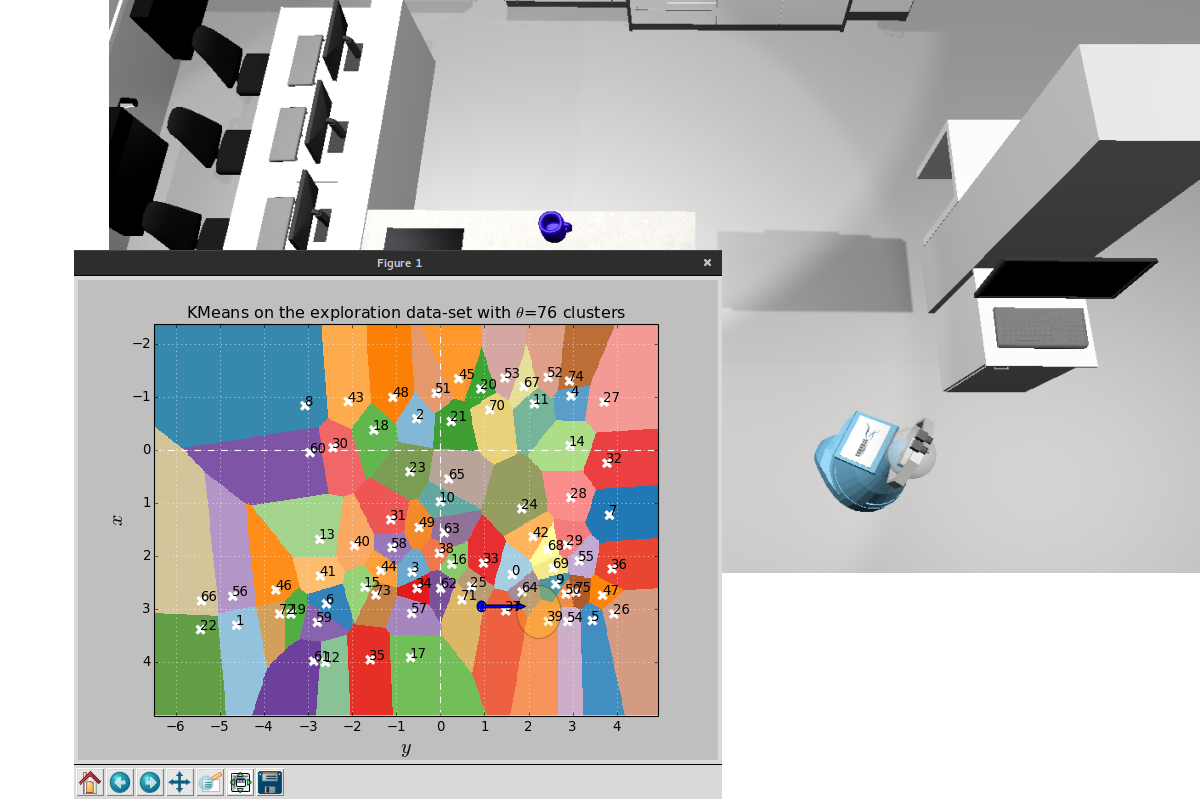
\includegraphics[width=\textwidth, left]{figures/simulation_learn_2}
%\end{column}
%\end{columns}
	
%\end{frame}

\begin{frame}
\frametitle{Model-Learning for Mobile Robot Navigation}
\framesubtitle{Learning State-Spaces}
\textbf{Given:} Execution trace(s) from exploration-stage 
\begin{columns}[T]
\begin{column}{0.4\textwidth}
	\vspace{12pt}
	\textbf{Existing Approaches:}
	\begin{itemize}
		\item \textcolor<2->{tudblue}{Grid-discretization}
		\item Best-First Model Merging
		\item State Merging by Trajectory Clustering
	\end{itemize}
	\pause
	\vspace{18pt}
	\small
	\only<3>{\textbf{Issues:} Dimensionality, \\\hspace{42pt}grid resolution}
\end{column}

\begin{column}{0.525\textwidth}
	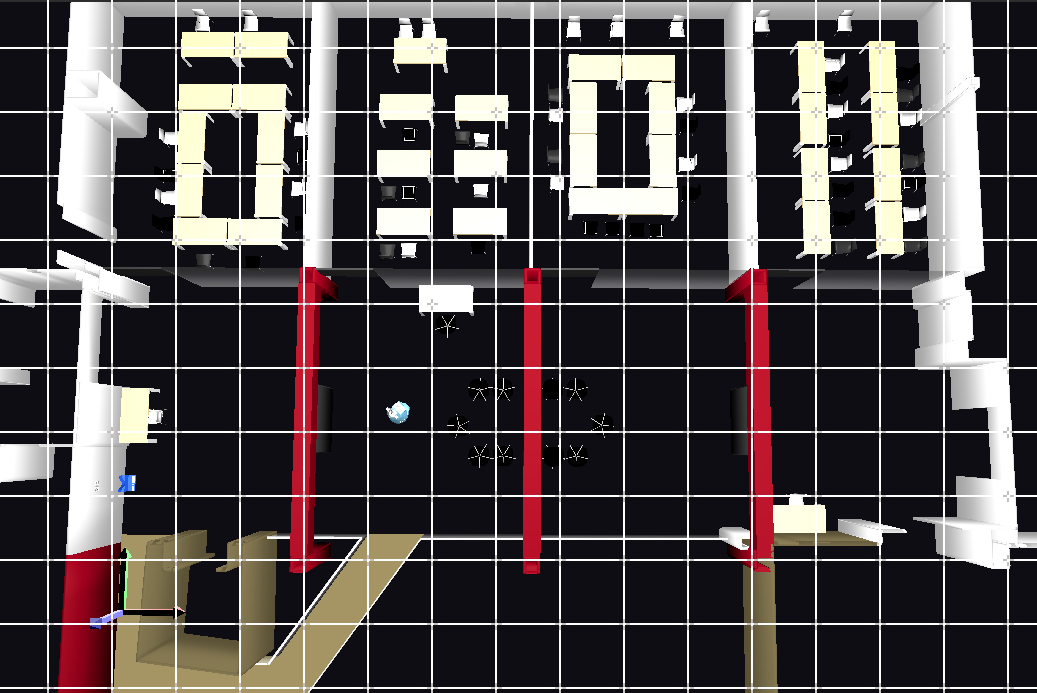
\includegraphics[width=\textwidth]{figures/simulator_topview_grid2}
\end{column}
\end{columns}

\end{frame}

\begin{frame}
	\frametitle{Model-Learning for Mobile Robot Navigation}
	\framesubtitle{Learning State-Spaces}
	\textbf{Given:} Execution trace(s) from exploration-stage 
	\begin{columns}[T]
		\begin{column}{0.4\textwidth}
			\vspace{12pt}
			\textbf{Existing Approaches:}
			\begin{itemize}
				\item Grid-discretization
				\item \textcolor{tudblue}{Best-First Model Merging}
				\item State Merging by Trajectory Clustering
			\end{itemize}
			\vspace{18pt}
			\small
			\only<2>{\textbf{Issues:} Greedy merging, \\\hspace{42pt}$O(t^3)$ algorithm}
		\end{column}
		\begin{column}{0.525\textwidth}
			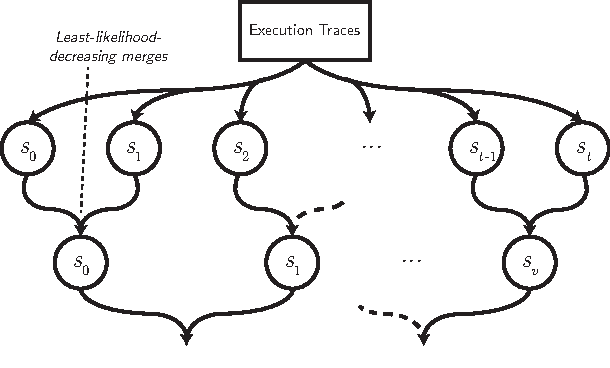
\includegraphics[width=1.11\textwidth]{figures/model-merging-bfmm}
		\end{column}
	\end{columns}
\end{frame}


\begin{frame}
	\frametitle{Model-Learning for Mobile Robot Navigation}
	\framesubtitle{Learning State-Spaces}
	\textbf{Given:} Execution trace(s) from exploration-stage
	\begin{columns}[T]
		\begin{column}{0.4\textwidth}
			\vspace{12pt}
			\textbf{Existing Approaches:}
			\begin{itemize}
				\item Grid-discretization
				\item Best-First Model Merging
				\item \textcolor{tudblue}{State Merging by Trajectory Clustering} % If we cluster states based on observations, for learning POMDPs we face the issue of perceptual aliasing -> to overcome this we do not look at the similarity in observations, but rather in the trajectories prior to these observations and do state merging of the time-states with the most similar trajectories
			\end{itemize}
			\vspace{18pt}
			\small
			\only<2>{\textbf{Note:} For learning POMDPs facing  \textit{perceptual aliasing}}
		\end{column}
		\begin{column}{0.525\textwidth}
			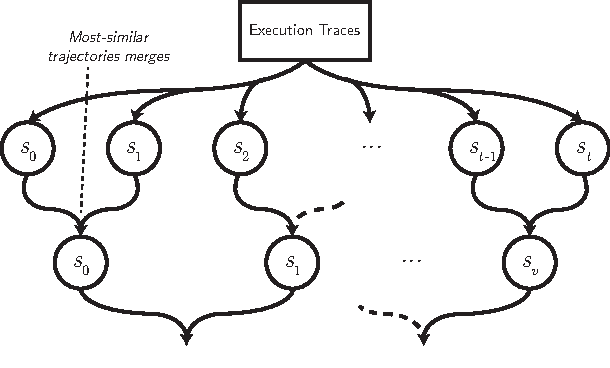
\includegraphics[width=1.11\textwidth]{figures/model-merging-trajectory}
		\end{column}
	\end{columns}
\end{frame}

\begin{frame}
	\frametitle{Model-Learning for Mobile Robot Navigation}
	\framesubtitle{Learning State-Spaces}
	\textbf{Given:} Execution trace(s) from exploration-stage

	\begin{columns}[T]
		\begin{column}{0.4\textwidth}
			\vspace{12pt}
			\pause
			\textbf{Approach:} Unsupervised ML for state-spaces, i.e.:
			\begin{itemize}
				\item<3-> K-Means Clustering
				\item<3-> Gaussian Mixture Models
				\item<3-> $\ldots$
			\end{itemize}
			\vspace{12pt}
			\only<4>{\textbf{Variable:} $\theta$ parameter of\\\hspace{50pt} ML-algorithm}
		\end{column}
		\begin{column}{0.525\textwidth}
			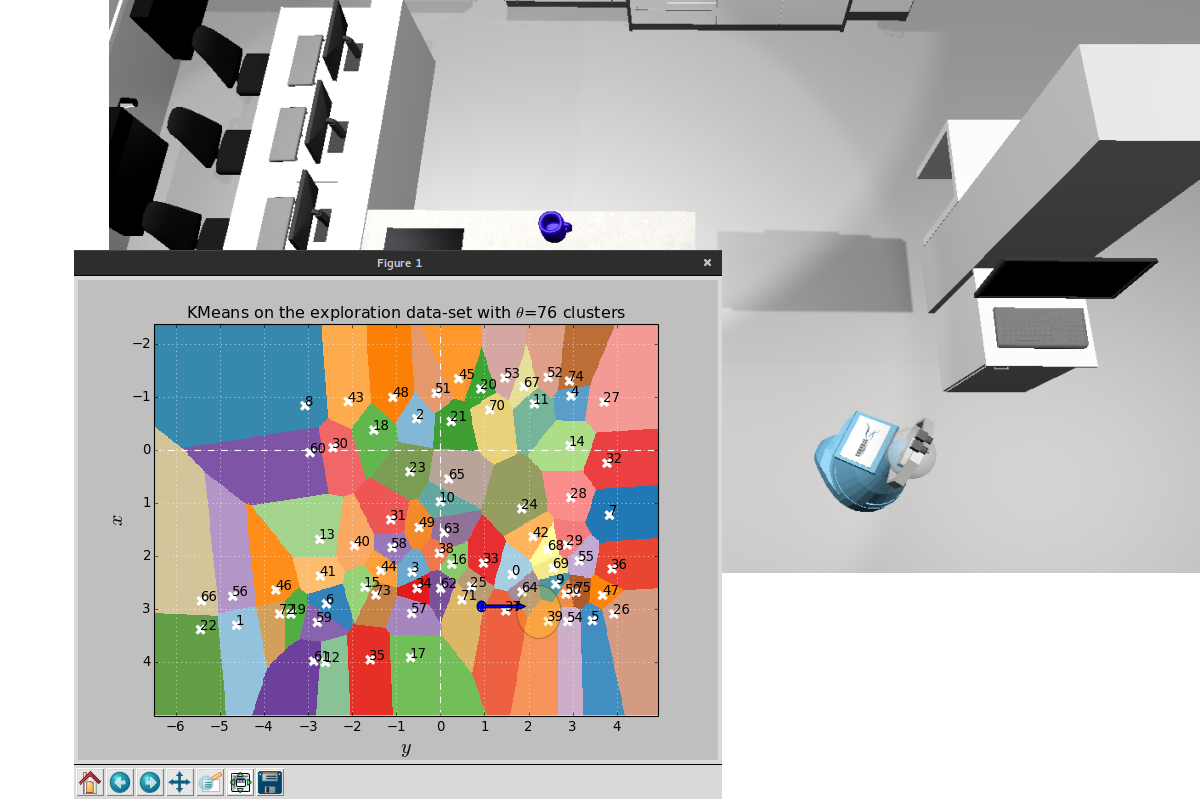
\includegraphics[width=1\textwidth]{figures/simulation_learn_2}
		\end{column}
	\end{columns}
\end{frame}

\begin{frame}
\frametitle{Model-Optimization Routine}
\begin{center}
\includegraphics<1| handout:0>[width=1\textwidth]{figures/optimization-routine/learning-cycle-1.pdf}
\includegraphics<2| handout:0>[width=1\textwidth]{figures/optimization-routine/learning-cycle-2.pdf}
\includegraphics<3| handout:0>[width=1\textwidth]{figures/optimization-routine/learning-cycle-3.pdf}
\includegraphics<4| handout:0>[width=1\textwidth]{figures/optimization-routine/learning-cycle-4.pdf}
\includegraphics<5>[width=1\textwidth]{figures/optimization-routine/learning-cycle-5.pdf}
\end{center}
\end{frame}

\begin{frame}
\frametitle{Model-Optimization Routine}
\begin{center}
	\includegraphics<1| handout:0>[width=1\textwidth]{figures/optimization-routine/learning-cycle-simplified-1.pdf}
	\includegraphics<2| handout:0>[width=1\textwidth]{figures/optimization-routine/learning-cycle-simplified-2.pdf}
	\includegraphics<3>[width=1\textwidth]{figures/optimization-routine/learning-cycle-simplified-v2-3.pdf}
\end{center}
\end{frame}